\subsection{Несинтаксические ограничения}
\MPS{} позволяет описывать различные несинтаксические ограничения моделей при помощи проблемно"=ориентированного языка \term{jet\-bra\-ins\-.mps\-.lang\-.const\-ra\-ints}. К таким ограничениям относятся: форматы значений свойств, функции вычисления синтетических свойств, области определения ссылок и ограничения на вложение одних узлов в другие.

Среда \MPS{} предоставляет всего три встроенных примитивных типа для свойств концептов: \term{string}, \term{boolean}, \term{integer}. Но при этом позволяет задать формат свойства и, таким образом, определить для свойства произвольный тип. Встроенный тип \term{string} разрешает использовать в качестве значения свойства любые строки. Для того, чтобы ограничить множество значений имен состояний только корректными \term{Java}-идентификаторами, концепт \term{AbstractState} реализует интерфейс"=концепт \term{IValidIdentifier}, который представляет собой раширение интерфейс"=концепта \term{INamedConcept} с соответствующим ограничением на свойство \term{name} (рис. \ref{fig:PropertyIsValid}).

\begin{figure}
 \centering
 \fbox{
  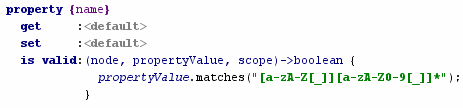
\includegraphics[width=0.8\textwidth]{PropertyIsValid.png}
 }
 \caption{Формат свойства \term{name} интерфейс"=концепта \term{IValidIdentifier}}
 \label{fig:PropertyIsValid}
\end{figure}

Любое свойство концепта может быть синтетическим, то есть вычислимым. Для этого достаточно задать функцию, вычисляющую значение этого свойства. Например, свойство \term{name} концепта \term{StateMachine} вычислимо. Его значение состоит из имени класса, автомат которого задает данный экземпляр \term{StateMachine}, и суффикса "<state machine"> (рис. \ref{fig:PropertyGet}).

\begin{figure}
 \centering
 \fbox{
  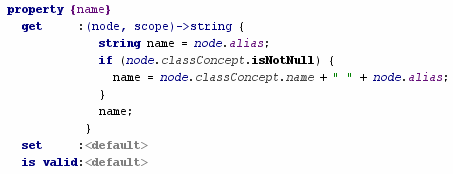
\includegraphics[width=0.8\textwidth]{PropertyGet.png}
 }
 \caption{Синтетическое свойство \term{name} концепта \term{StateMachine}}
 \label{fig:PropertyGet}
\end{figure}
